\section{Method}
\label{sec:method}
In order to answer the research questions stated in section~\ref{sec:RQ}, a state of the art SPC, experiments and evaluation methods needs to be set up. In this section all the necessary hardware and software components and theory will be presented as well as the evaluation techniques. 


\subsection{Single pixel camera architecture \& hardware}
\label{sec:system}
FOI designed the SWIR SPC platform using a DMD, a Newtonian telescope and a single pixel SWIR detector. The system also has a reference camera in the visual spectrum  which can capture images of the scene reflected on the DMD, check that the patterns are displayed correct on the DMD and simplifying focusing of the image.  

\begin{figure}[H]
    \centering
    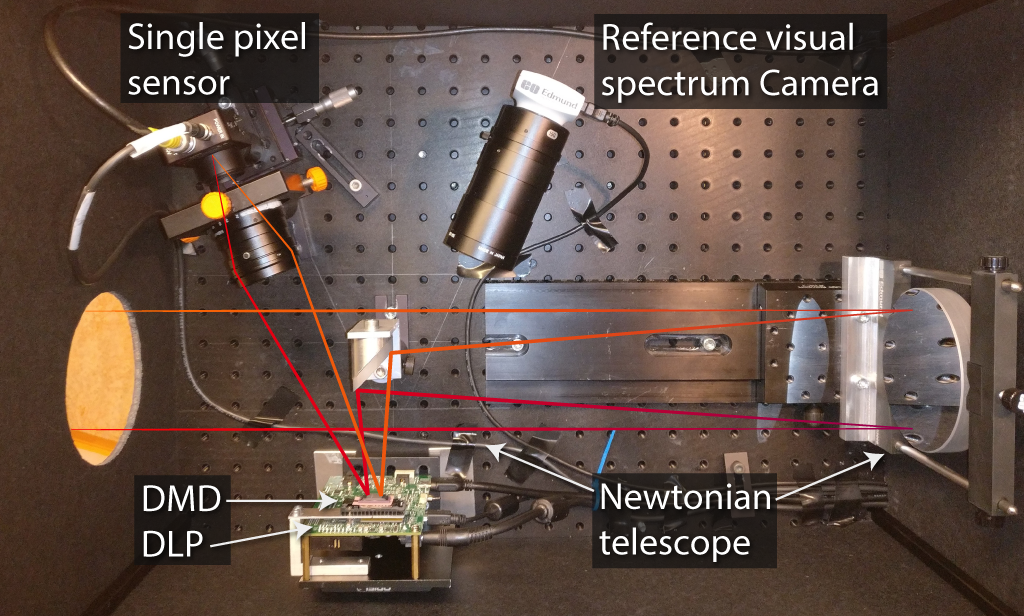
\includegraphics[width = 0.9\textwidth]{gfx/SPC.png}
    \caption{The single pixel camera architecture used in this thesis. In the image, the aperture, reflective optics, DMD, reference camera and the single pixel sensor are shown from an areal view including red lines showing the incoming light path.}
    \label{fig:system1}
\end{figure}



As seen in figure~\ref{fig:system1}, light from the scene is focused by the Newtonian telescope and reflected onto the DMD. The mirrors on the DMD can reflect the light individually either into the single pixel sensor or the reference camera. The DMD acts as a Spatial Light Modulator (SLM) and reflects different patterns which is 'summed up' in the single pixel sensor as a voltage intensity. The reconstructed image from the system will have the same resolution as the DMD patterns. The digital light processor (DLP) is the DMD:s control unit which controls which patterns are displayed on the DMD either by reading images from memory or the HDMI video port. 

\subsubsection{Newtonian telescope}
A Newtonian telescope is a reflecting telescope, using a concave primary mirror and a flat diagonal secondary mirror, see figure~\ref{fig:system1}. In this set-up the telescope act as a lens focusing the scene onto the DMD. The motivation to use a Newtonian telescope instead of a lens system is partly that chromatic aberration is eliminated and partly that a reflective optical system works over a greater range of wavelengths that includes SWIR, near infrared (NIR) and the visible spectrum. This design has a very narrow field of view which give high detailed scenes from a great distance. 


\subsubsection{DLP and DMD}
The DMD (Texas Instruments DLP4500NIR) is a matrix of micro mirrors that can be individually tilted $\pm 12^{\circ}$ and reflects wavelengths in the range 700-2500 nm. The DMD is controlled by the DLP (DLP\textregistered ~LightCrafter\textsuperscript{TM} 4500) which can be controlled either by video port (HDMI) or by the internal flash memory. The internal memory can theoretically be faster than the video port, but due to constraints in both memory and memory bandwidth, the fastest measurement matrix rate gets stuck at $270 - 300$ Hz. The video port can be operated at 120 Hz and display one bit plane at the time from a $24$ bit signal, which gives a maximum measurement matrix rate at $120 \times 24 = 2880$ Hz, but in the current configuration only $60$ Hz frame rate was achieved giving a measurement matrix rate at $1440$ Hz. At this rate with subsampling ratio (the number of measurements relative number of pixels) between $20\% - 30\%$ with $512\times512$ pixel images, the sampling would be acquired in $36 - 52$ seconds. To control the DMD the software "DLP LightCrafter 4500 Control Software" is used.\cite{manual:DLP}\\[0.1in] 

The DMD used in the setup is constructed with a diamond shaped pattern instead of a regular square grid which is used in regular camera image sensors. The diamond shape causes the index of each mirror to be skewed against what a normal grid would look like. As seen in figure~\ref{fig:dmd_index}, the indexes of the mirrors column is two mirror column arrays wide while a row is a single row. 


\begin{figure}[H]
    \centering
    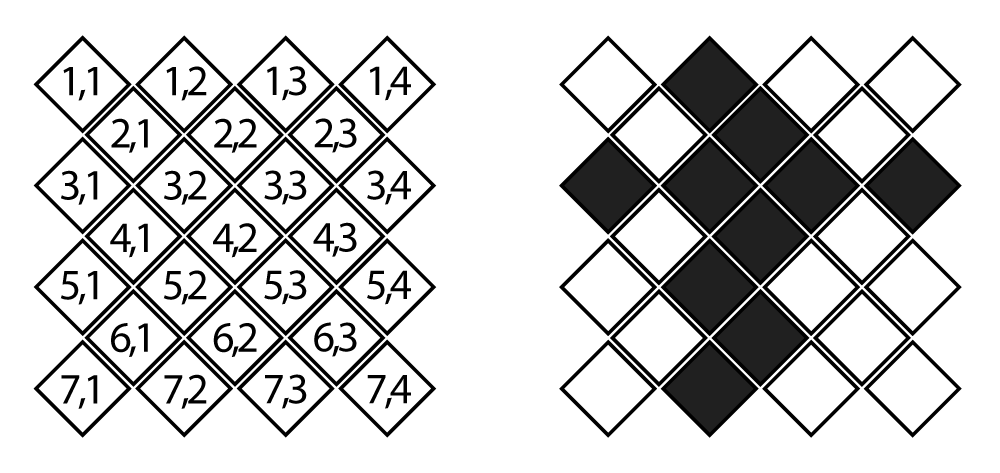
\includegraphics[width = 0.8\textwidth]{gfx/DMD_grid.png}
    \caption{DMD matrix mirror index, left shows each tiles index and right shows the second row and second column in black as set by default from the factory.}
    \label{fig:dmd_index}
\end{figure}

Because the reconstruction algorithm and measurement matrix needs to be a square matrix with the side length with a power of 2, the resulting images ratio would be 2 to 1, while the image should have the ratio 1 to 1. The resulting image would need to be transformed into the real ratio where information potentially gets lost. Therefore the index of mirrors was changed so that each 'pixel' gets two mirrors as seen in figure~\ref{fig:dmd_index2}. This will result in rows and columns gets equal amount of space and the aspect ratio will be preserved 1 to 1. By grouping two mirrors, the amount of light from each "pixel" is doubled and thus should improve the sampled signal quality.

\begin{figure}[H]
    \centering
    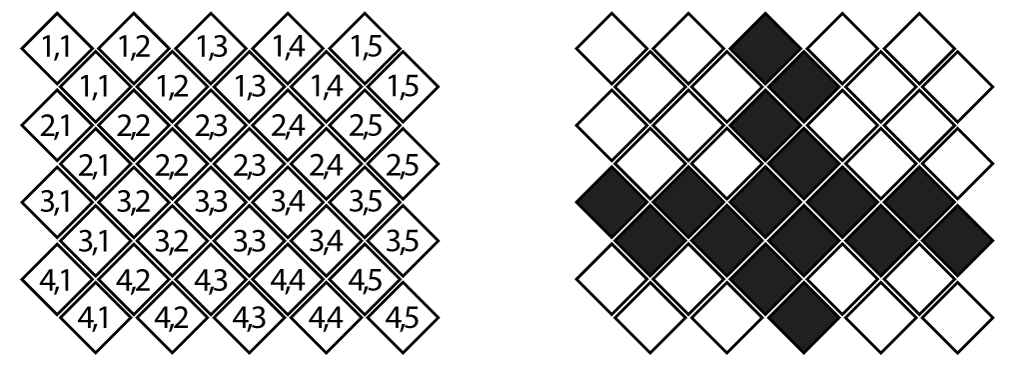
\includegraphics[width = 0.8\textwidth]{gfx/DMD_grid2.png}
    \caption{DMD matrix, left shows each tiles index and right shows third row and third column in black.}
    \label{fig:dmd_index2}
\end{figure}

Mathematically the DMD is a binary operator which lets light pass or not, in figure~\ref{fig:dmd_pattern} a typical pattern that could be sent to the DMD is shown.  

\begin{figure}[H]
    \centering
    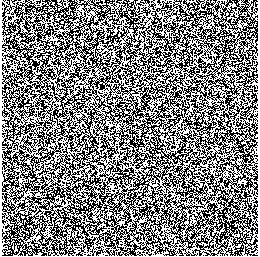
\includegraphics[width = 0.5\textwidth]{gfx/DMD_pattern.png}
    \caption{A typical pseudo random measurement matrix sent to the DMD with the resolution $256 \times 256$ pixels.}
    \label{fig:dmd_pattern}
\end{figure}



\subsubsection{Lens}
The lens mounted on the single pixel sensor is a 50 mm SWIR Fixed Focal Length Lens with a variable aperture from f-stop f/1.4 designed for wavelengths ranging from the 800 nm in the visual spectrum to 2000 nm in the SWIR spectrum. \cite{website:SWIR_objective}

\subsubsection{Single pixel sensor}
The single pixel sensor is a Thorlabs PDA20C/M and is sensitive in wavelength range 800-1700 nm which is beyond the visual spectrum (390-700 nm). The sensors built-in amplifier outputs an analog signal in volt which the sampler converts to a discrete value. \cite{manual:PDA}

\subsubsection{Signal spectrum}
All components characteristics assembled, the wavelengths that pass trough the system and measured in the single pixel sensor is between 800-1700 nm.



\subsection{Compressive imaging}
\label{sec:CI}
Compressive imaging is the name used when sampling and reconstructing images using the compressive sensing method. CI is often realized in form of a SPC but can have different shapes. In this thesis CI is used on the SPC architecture presented in section~\ref{sec:system}. CI exploits the fact that natural images are compressible or approximately sparse in some basis and therefore only a few measurements relative to the image pixel resolution needs to be measured in order to reconstruct the image.\\[0.1in]

CI need to fulfill two constraints in order to utilize CS sampling,  the image needs to be compressible and the complete measurement matrix need to be incoherent with the sparse transform. The first constraint is fulfilled because it is known that natural images are compressible using for example JPEG (using Discrete cosine transform) or JPEG2000 (using wavelet transform) and the second constraint is fulfilled using a measurement matrix with a random characteristic and will be explained further in section~\ref{sec:mm_RIP}.\\[0.1in]
 

The single pixel sensor captures a scene by measuring the light intensity focused onto the detector reflected from the DMD pattern. The DMD pattern changes to obtain new measurements. $M$  measurements are sampled to reconstruct an image with $N$ pixels, where $M \ll N$. Each measurement matrix index is encoded either  by a one or a zero (turning the mirror onto or away from the sensor).\\[0.1in] 

The compressive imaging sampling model is defined as

\begin{equation}
\label{eq:CS1}
   \mathbf{ y = \Phi x + \epsilon}\text{,}
\end{equation}\\[0.1in]


where $\mathbf{x}_{N\times1}$ is the image rearranged as an array with $N$ pixels, $\mathbf{y}_{M\times1}$ is the sampled signal with $M$ measurements, $\mathbf{\Phi}_{M \times N}$ is the complete measurements matrix and $\mathbf{\epsilon}$ is the noise.\\[0.1in] 

In this thesis $\mathbf{\Phi}$ is defined as the \textit{complete measurement matrix} and mainly used in mathematical context, the rows of the complete measurement matrix contains the \textit{measurement matrices}, where one measurement matrix is denoted $\mathbf{\phi}_m$ but can also be denoted as \textit{DMD patterns}. The complete measurement matrix thus contains $M$ measurement matrices.\\[0.1in]


In conventional sampling the number of measurements $M$ needs to be at least equal to the number of pixels $N$ in the image to recover the signal, but CS states that $M$ can be relatively small compared to $N$ given how compressible the image is. This is because the image $\mathbf{x}$ can be represented as  

\begin{equation}
\label{eq:CS2}
   \mathbf{ \Psi \theta = x }\text{,}
\end{equation}\\[0.1in]

where, $\mathbf{\Psi}_{N \times N}$ is some basis matrix and
$\mathbf{\theta}_{N\times1}$ is the coefficients where $\mathbf{\theta}$ is $K$-sparse. $K$-sparse means that the image $\mathbf{x}$ has $K$ non zero elements in basis $\mathbf{\Psi}$, $||\mathbf{\theta}||_0 = K$. Given~(\ref{eq:CS2}), (\ref{eq:CS1}) can be expanded to


\begin{equation}
   \mathbf{ y = \Phi x + \epsilon = \Phi \Psi \theta + \epsilon = A \theta + \epsilon }\text{,}
   \label{eq:CS}
\end{equation}\\[0.1in]

where, $\textbf{A}_{M \times N} = \mathbf{\Phi \Psi}$ is called the reconstruction matrix.\\[0.1in] 

The revelation in~(\ref{eq:CS}) is what makes CS powerful. By sampling the scene using the complete measurement matrix $\mathbf{\Phi}$ (as~(\ref{eq:CS1})) but then in the reconstruction process transforming the complete measurement matrix $\mathbf{\Phi}$ to the reconstruction matrix $\mathbf{A}$ using some basis $\mathbf{\Psi}$, the optimization algorithm can solve the system for the sparse coefficients $\theta$ instead of the spatial image coefficients in $\mathbf{x}$ which are not sparse.\cite{book:sm}\\[0.1in]

A great advantage CI has over regular cameras, where each pixel is sampled separately, is that roughly half the pixels is sampled in one sensor, meaning that background noise of the sensor will be surpassed by the summed intensity of half the pixels making CI very robust to noise.  


\subsection{Measurement matrix and Restricted isometry property (RIP)}
\label{sec:mm_RIP}
As stated in section~\ref{sec:CI}, the complete measurement matrix needs to be incoherent with the sparse transform. In this section the most powerful constraint on a complete measurement matrix is shown, the restricted isometry property (RIP). \\[0.1in]

In the noiseless case exact recovery of the image $\mathbf{x}$ is achievable if RIP holds for the reconstruction matrix $\mathbf{\Phi} \Rightarrow \mathbf{\Phi\Psi = A}$, the constraint is defined as,

\begin{equation}
    (1-\delta_K)||\mathbf{x}||_{\ell_2}^2\leq||\mathbf{Ax}||_{\ell_2}^2\leq(1+\delta_K)||\mathbf{x}||_{\ell_2}^2 \text{,}
\end{equation}\\[0.1in]

where $\delta_K \in [0.1)$ is the smallest constant to satisfy RIP for a K-sparse signal $\mathbf{x}$. To determine a sampling matrix is a NP-hard problem (which means that there is no feasible way of creating a optimal reconstruction matrix) and generally $\textbf{x}$ is not known and varies, which means that there are no general optimal reconstruction matrices for natural images. Therefore, it is desired to find a general reconstruction matrix that satisfies RIP with high probability. It has been proved that constructing the complete measurement matrix by picking independent and identically distributed (i.i.d.) random variables gives $\delta_K << 1$ with high probability. Constructing the measurement matrices using i.i.d random variables has showed that the number of measurements $M$ needed to satisfy RIP with high probability is $M \geq O(K\text{log}(N/K) \ll N$. \cite{book:srr}\\[0.1in]

The problem of using random matrices is that they need to be stored in memory for the reconstruction algorithm, so when the image resolution is increased the measurement matrix increases exponentially. For images with resolution of $512\times 512$ and larger, the data gets unfeasible for a normal computer to handle.\\[0.1in]  

Fortunately, by changing the complete measurement matrix to structurally random matrices, fast transforms can be used in the reconstruction algorithm instead of vector multiplication, resulting in both faster reconstruction and the need to store the measurement matrix in memory. In this thesis, the permutated sequency ordered Walsh Hadamard measurement matrix (described in section~\ref{sec:SOWHMM}) will be used with the TVAL3 reconstruction algorithm (described in section~\ref{sec:TV}) to achieve higher resolution photos and faster reconstruction.   


\subsubsection{Permutated sequency ordered Walsh Hadamard measurement matrix}
\label{sec:SOWHMM}
Besides from eliminating the need to store the measuring matrix in computer memory for reconstruction, the permutated sequency ordered Walsh Hadamard matrix (PSOWHM) can be generated when sent to the DMD and thus eliminating the need to store the matrix at all. PSOWHM has approximatly the same characteristics and properties as an i.i.d. random matrix but generally has a higher number of measurements for exact reconstruction of the image, $M \sim (KNs)\log^2(N)$, where $s$ is the average number of non zero indexes in the measurement matrix \cite{lec:fast_CS_SRM}. Research has however shown that there is no significant loss in recovery of the image relative the i.i.d. random measurement matrix~\cite{article:an_improved_WH_matrix}. An other property of PSOWHM is that it only contains -1 and 1, which can easily be converted to 0 and 1 when sent to the DMD. \\[0.1in]


In order to construct the PSOWHM, the fist step is to define the naturally ordered Hadamard matrix and then follow a few additional steps. The naturally ordered Hadamard matrix of dimension $2^k$, $k \in \mathbb{N}$ is constructed by the recursive formula    

\begin{equation}
    H_0 = 1,
\end{equation}

\begin{equation}
    H_1 = \begin{bmatrix}
       1 & 1 \\
       1 & -1\\
     \end{bmatrix},
\end{equation}

and in general,

\begin{equation}
        H_k = \begin{bmatrix}
       H_{k-1} & H_{k-1} \\
       H_{k-1} & -H_{k-1}\\
       \end{bmatrix} = H_1 \otimes H_{k-1}
\end{equation}

where $\otimes$ denotes the Kronecker product.\\[0.1in]

To construct the permutated sequency ordered Walsh Hadamard matrix from the naturally ordered Hadamard matrix these steps are required:

\begin{itemize}
    \item Convert row index $n_H$ to binary.
    \item Convert the binary row index to Gray code.
    \item Apply bit reverse on the Gray code index.
    \item Remove first row with only ones.
    \item Permutate columns and choose $M$ rows at random.
\end{itemize}

Then order the rows after the bit-reverse to obtain the sequency ordered Walsh Hadamard matrix.

\begin{table}[H]
\begin{tabular}{|r|c|c|c|c|}
\hline
    $n_H$        & 0    & 1     & 2     & 3     \\ \hline
    Binary       & 00   & 01    & 10    & 11    \\ \hline
    Gray code    & 00   & 01    & 11    & 10    \\ \hline
    Bit-reverse  & 00   & 10    & 11    & 01    \\ \hline
    $n_W$        & 0    & 2     & 3     & 1     \\ \hline
    
\end{tabular}
	\label{tab:Hadamard_2_Walsh}
	\caption{Example how to convert a naturally ordered Hadamard matrix to a sequency ordered Walsh Hadamard matrix by shifting row with index $n_W$ to $n_H$}
\end{table}

for example

\begin{equation}
    H_2 =  \begin{bmatrix}
       1 & 1 & 1 & 1 \\
       1 & -1 & 1 & -1 \\
       1 & 1 & -1 & -1 \\
       1 & -1 & -1 & 1 
       \end{bmatrix} \Rightarrow W_2 = \begin{bmatrix}
       1 & 1 & 1 & 1 \\
       1 & 1 & -1 & -1  \\
       1 & -1 & -1 & 1  \\
       1 & -1 & 1 & -1 
       \end{bmatrix}.
\end{equation}

To use the sequency ordered Walsh Hadamard matrix as a measurement matrix the first row is omitted, permutations to the columns are performed, $M$ rows are choosen at random and the indices with $-1$ shifted to $0$. How the matrix are permutated and which rows are choosen in which order are stored so the reconstruction algorithm can use that information to reverese the process. This method is used to distribute the energy of the signal's sample across all measurements.   \cite{article:SRM_long, article:TVAL3, article:an_improved_WH_matrix}. 


\subsection{Reconstruction method}
To reconstruct the image $\textbf{x}$, the sparsest set of coefficients in $\theta$ is desired. The optimal approach to find these coefficients would be to use $\ell_0$ minimization


\begin{equation}
   \mathbf{ \hat{\theta}} = \text{arg min } ||\mathbf{\theta}||_0 \text{  subject to  } \mathbf{y = A\theta} \text{.}
\end{equation}\\[0.1in]


This seems simply to be minimizing nonzero indices in $\mathbf{\theta}$ in the sparsifying basis $\mathbf{\Psi}$, but this problem is known to be NP-hard. A better approach is the $\ell_1$ minimization, for example Basis Pursuit denoise (BPDN),

\begin{equation}
    \mathbf{\hat{\theta}} = \text{arg min } ||\mathbf{\theta}||_1 \text{  subject to  } ||\mathbf{y - A\theta}||_2 < \mathbf{\epsilon} \text{.}
\end{equation}\\[0.1in]


In 2006 Donoho~\cite{article:CS_donoho1} for the first time guarantied theoretical $\ell_0\text{/}\ell_1$ equivalence which holds in the CS case, which means using a $\ell_1$ minimizer is guaranteed to find the sparsest solution in polynomial time in the noiseless case which can be approximated in the noisy and compressible signal case. The drawback with the $\ell_1$ minimizer is that it requires more measurements than the optimal case with $\ell_0$ but $M \ll N$ still holds. Since 2006 many more types of optimization algorithms have evolved which solves the problem with different methods but with the same goal: finding the largest, most significant coefficients of $\mathbf{\theta}$. \cite{article:CS_donoho1, article:single_pixel_im_cs, article:a_new_ci_arc}


\subsubsection{Total variation: TVAL3}
\label{sec:TV}
The reconstruction algorithm that was chosen in this thesis was a total variation (TV) regularization algorithm called TVAL3 and was chosen for its speed and good results in image reconstruction compared to other reconstruction algorithms created for the CS problem \cite{article:TVAL3}. Natural images often contains sharp edges and piecewise smooth areas which the TV regularization algorithm is good at preserving. The main difference between TV and other reconstruction algorithms is that TV considers the gradient of signal to be sparse instead of the signal itself, thus finding the sparsest gradient. 

The TV optimization problem in TVAL3 is defined as  

\begin{equation}
\text{min}_\mathbf{x} \Sigma_i ||D_i \mathbf{x} || \text{, subject to } \mathbf{\Phi x} = 	y \text{, } \mathbf{x} \geq 0 \text{,} 
\label{eq:tval3}
\end{equation}

where $D_i\mathbf{x}$ is the discrete gradient of $\mathbf{x}$ at position $i$.\\[0.1in]

TVAL3 stands for "Total Variation Augmented Lagrangian Alternating Direction Algorithm", where augmented Lagrangian is a method in optimization for solving constrained problems by substituting the original constrained problem with a series of unconstrained subproblems and introducing a penalty term. To solve the new subproblems the alterning direction method is used~\cite{article:TVAL3}.\\[0.1in]

As mentioned earlier in section~\ref{sec:SOWHMM}, the main reason to use the permutated sequency ordered Walsh Hadamard matrix is to eliminate the need to store the matrix in computer memory during reconstruction and to speed up the reconstruction. In TVAL3 there are two multiplications between matrix and a vector that dominates the computation time,

\begin{equation}
\mathbf{\Phi}\mathbf{x}^k \text{ and } \mathbf{\Phi}^\top(\mathbf{\Phi}\mathbf{x}^k-\mathbf{y})\text{.}
\end{equation}

The idea is to replace the multiplication with fast transforms. To explain the concept some observations and new functions need to be defined. The first observation is that the sequency ordered Walsh Hadamard matrix is a transform matrix, which also can be computed with the fast Walsh Hadamard transform (FWHT),

\begin{equation}
\mathbf{W}\mathbf{x} = \text{ FWHT}(\mathbf{x}),
\label{eq:fwht}
\end{equation}

where $W$ is a sequency ordered Walsh Hadamard matrix and $\mathbf{x}$ is the image vector. The Walsh Hadamard transform (WHT) is a generalized class of Fourier transforms, which decomposes the input vector into superposition of Walsh functions.\\[0.1in]

In section~\ref{sec:SOWHMM} it was briefly mentioned in the last paragraph that the measurement matrix columns is permutated and rows are chosen at random to create the measurement matrix from the sequency ordered Walsh Hadamard matrix. To describe the different permutations two functions is defined.\\[0.1in] 

\theoremstyle{definition}
\begin{definition}{Column permutation operator}
$\pi(\cdot)$, permutates the order of the columns in a matrix or a vector from a random seed.
\label{def:col_perm}
\end{definition}

\theoremstyle{definition}
\begin{definition}{Subsampling matrix operator}
$\Pi_M(\cdot)$ chooses $M$ row in a matrix at random and stacks them in a new matrix.
\label{def:subsamp_perm}
\end{definition}


Now the complete measurement matrix $\mathbf{\Phi}$ can be constructed using the sequency ordered Walsh Hadamard matrix, statement in equation~\ref{eq:fwht}, definition~\ref{def:col_perm} and \ref{def:subsamp_perm},


\begin{equation}
\mathbf{\Phi} = \pi(\Pi_M(\mathbf{W})) = \Pi_M(\pi(\mathbf{W}))\text{.}
\end{equation}

Note that it does not matter in which order the functions are applied, it gives the same result. Also note that multiplication between a matrix and a vector where one of the variables has been permuted by $\pi(\cdot)$, the function can change variable without changing the result since,

\begin{equation}
\pi(\mathbf{\Phi})\mathbf{x} = \mathbf{\Phi}\pi(\mathbf{x})\text{.}
\label{eq:pi_trans}
\end{equation}


With all observations combined, the matrix multiplication is replaced with the FWHT and operators in definition~\ref{def:col_perm} and \ref{def:subsamp_perm} as shown in equation~\ref{eq:fwht_def},

\begin{equation}
\mathbf{y} = \mathbf{\Phi}\mathbf{x} = \pi(\Pi_M(\mathbf{W}))\mathbf{x} = \Pi_M(\mathbf{W})\pi(\mathbf{x}) = \Pi_M(\mathbf{W}\pi(\mathbf{x})) = \Pi_M(\text{FWHT}(\pi(\mathbf{x}))\text{.}
\label{eq:fwht_def}
\end{equation}

Using this method will reduce the overall computational complexity considerably and it will make the measurement matrix redundant in the reconstruction. Only the two permutation functions $\pi(\cdot) \text{ and } \Pi_M(\cdot)$ needs to be stored. Eliminating the need of the complete measurement matrix in the reconstruction unlocks the potential to reconstruct images with high resolution ($512\times512$ pixels and larger). \cite{article:SRM_long, article:TVAL3}



\subsection{Image Capturing and processing chain}
\label{sec:image_capturing_and_process_chain}
In figure~\ref{fig:flow_chart} the whole process of capturing an image is presented with all subsystems and signal/image processing steps included.

\begin{figure}[H]
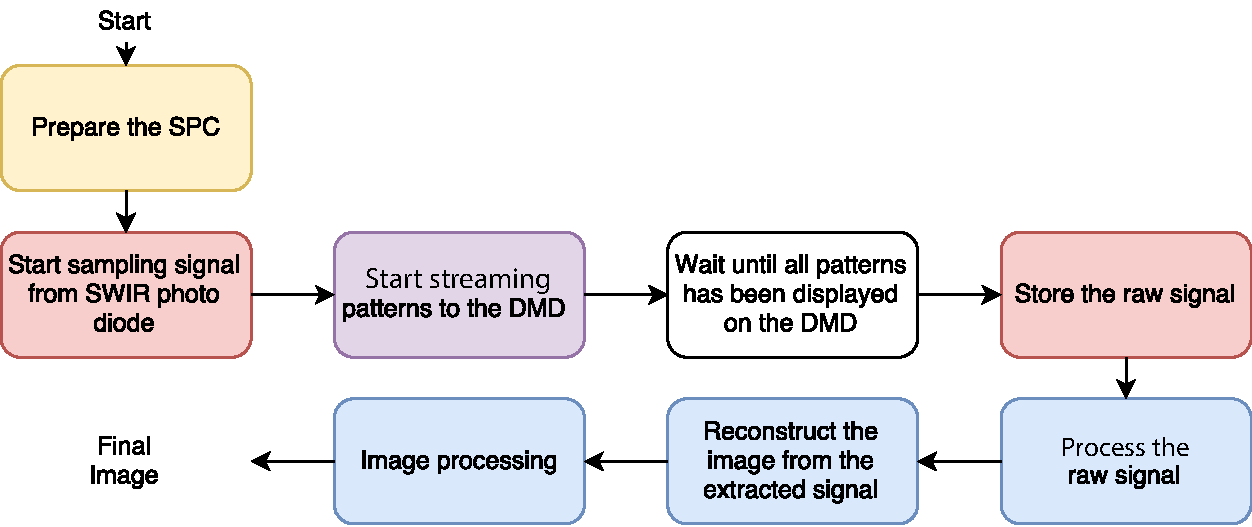
\includegraphics[width = 1\linewidth]{gfx/flowchart3.pdf}
\caption{Block diagram of image capturing and processing chain, from signal acquisition to final image. Each color represents different subsystems in hardware or software (described in section~\ref{sec:p_spc}-\ref{sec:ip}).}
	\label{fig:flow_chart}
\end{figure}

This experimental setup is not a fully automatic system where a button can be pressed and the system produces an image. In the setup the subsystems works completely independently and needs to be operated manually in the right order at the right time. Each color in figure~\ref{fig:flow_chart} represents a subsystem in hardware or software. Each subsystem is described in the following subsections.

 
\subsubsection{Prepare the SPC}
\label{sec:p_spc}
The first step in the yellow block "Prepare the SPC" (figure~\ref{fig:flow_chart}) is to make sure that the SPC is up and running but also to point the camera at the scene and set the correct focus. The scene is located with the aid of the reference camera (see figure~\ref{fig:system1}), with all the mirrors in the DMD directed to that camera. The focus is adjusted manually by moving the primary mirror back or forth, this procedure may introduce some error to the focus.\\[0.1in]

\subsubsection{Sampling}
The red blocks subsystem "Start sampling signal from SWIR photo diode" and "Store the raw signal" (figure~\ref{fig:flow_chart}) is conducted in a separate software which controls the A/D converter and thus the sampling. When the SPC is prepared, the sampling of the signal is started with a sampling rate such that every measurement has several sampling points and thus over-samples the signal. The oversampling is needed because when the mirrors move from one pattern to the next, the signal is uncertain for some time. The oversampling is also used to suppress noise from the photo diode (see further section~\ref{sec:signal_process}). After the signal is sampled the obtained signal is stored on the computer manually.

\subsubsection{Streaming patterns to the DMD}
\label{sec:stream_dmd}
The subsystem "Streaming patterns to the DMD" (figure~\ref{fig:flow_chart}), represented in the purple block, is controlled by two different softwares, one which manipulates the pattern-signal received by the DMD and one which sends the patterns to the DMD. The patterns are sent to the DMD through a HDMI cable where the DMD is set up such that the DMD acts as a second screen to the computer. This enables to show anything on the DMD that the screen can show. The patterns are stored as a video and played back on the DMD "screen" with a media player, which shows each pattern in consecutive order. This is the major bottleneck of the system where each measurement matrix needs to be displayed one after the other depending on how fast frame rate that can be achieved. The naive approach would be to display one pattern per frame which is linked to the frame rate of the DMD. For example, 60 frames per second (fps). For a $512\times 512$ image subsampled at $20\%$ which corresponds to $512\times 512 \times 0.2 = 52429$ patterns which would take $52429/60 = 874 \text{ seconds} = 14.5 \text{ minutes}$ to sample. This is a long exposure time for a still image with the constraint that the scene should be stationary to obtain a stationary signal.\\[0.1in]

Fortunately, with the software "DLP LightCrafter 4500 EVM GUI" controlling the DMD, the received video signal can be manipulated before displayed onto the DMD. The software includes a function which can break down the received 24-bit color image into 1 bit planes which can be displayed in consecutive order. This function improves the naive implementation by a factor of $24$, which reduces the time to sample the image in the given example from $874 \text{ seconds to } 874/24 = 36 \text{ seconds}$. That long exposure time is of course not optimal for natural images outdoors, but acceptable for the experimental setup.\\[0.1in]     


To create the video that feeds the patterns to the DMD each pattern,  i.e. measurement matrix, is created as presented in section~\ref{sec:SOWHMM}. Then each group of 8 unique patterns are stacked in the 8 bit planes of an 8 bit image as seen in figure~\ref{fig:8_to_1_8}.

\begin{figure}[H]
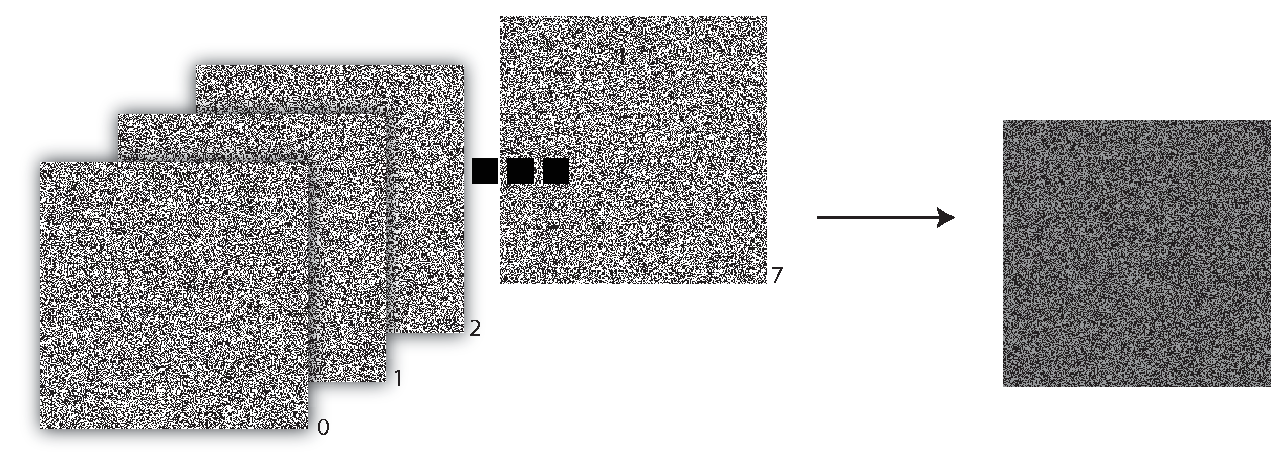
\includegraphics[width = 1\linewidth]{gfx/DMD_12.eps}
\caption{Each group of 8 measurement matrices is stored in separate  bit planes in one 8 bit image.}
	\label{fig:8_to_1_8}
\end{figure}

Then for each group of three 8 bit images a 24 bit color image is constructed as seen in figure~\ref{fig:3_8_to_1_3}. 

\begin{figure}[H]
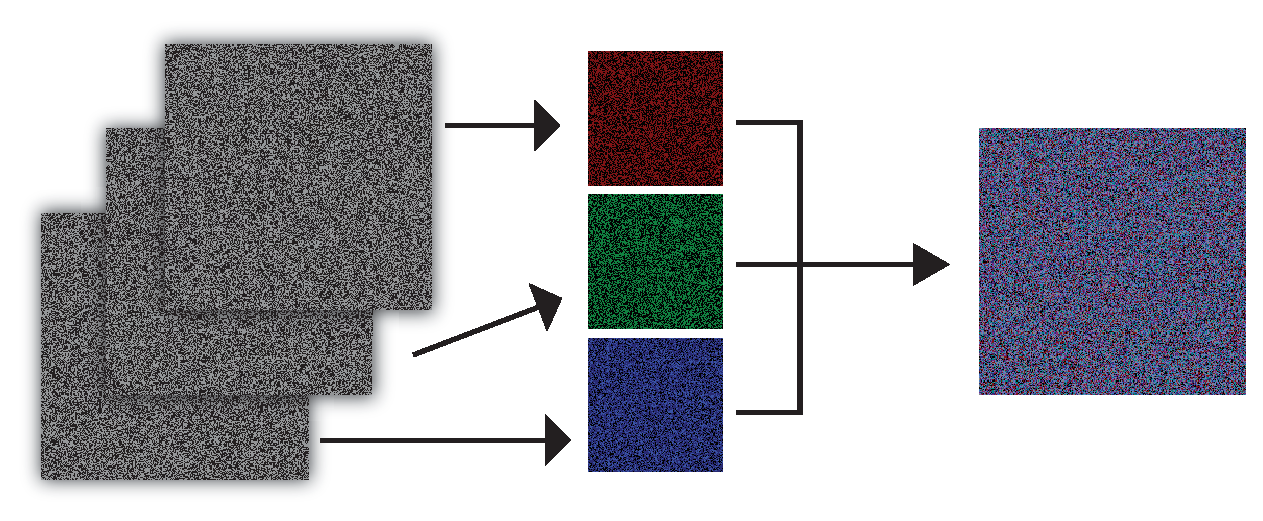
\includegraphics[width = 1\linewidth]{gfx/DMD_2.eps}
\caption{Each group of three 8 bit images is stored into one 24 bit color image. This is one frame in the video sent to the DMD.}
	\label{fig:3_8_to_1_3}
\end{figure}

The 24 bit color image corresponds to one frame in the video.



\subsubsection{Signal processing}
\label{sec:signal_process}  
When the sampled signal is stored in the computer the remaining signal/image processing and reconstruction represented by blue blocks in figure~\ref{fig:flow_chart} is conducted in MATLAB. In this section the signal processing of the sampled signal is described.\\[0.1in]

The first step is to refine the raw over-sampled signal so that each measurement matrix corresponds to one measurement in signal $\mathbf{y}$. This is done by first finding every set of indices that correspond to every measurement matrix, see figure~\ref{fig:raw_signal} where the signal indices are isolated by the magenta lines.


\begin{figure}[H]
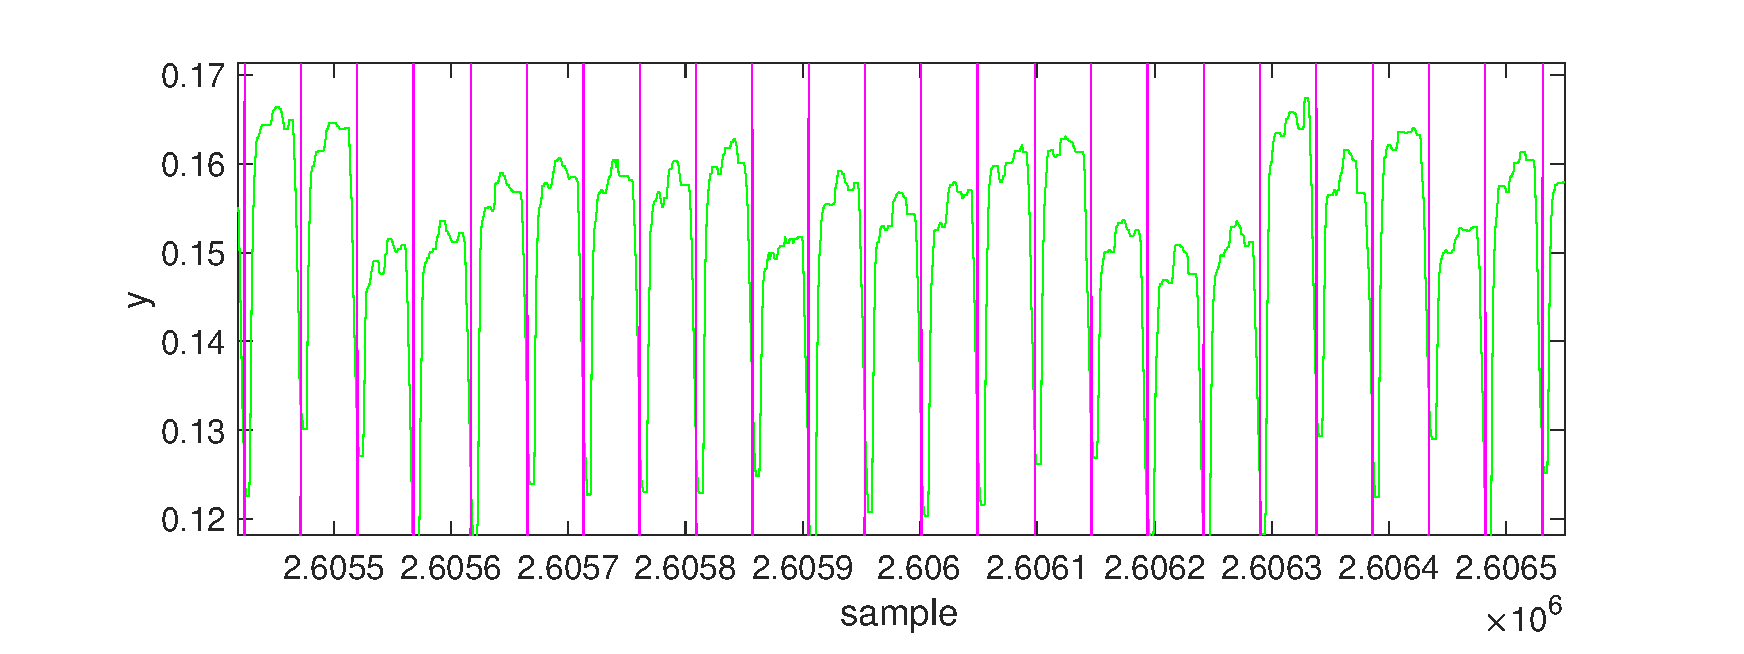
\includegraphics[width = 1\linewidth]{gfx/signal_proc/isolated_raw_signal.eps}
\caption{A simulated noisy over-sampled signal $\mathbf{y}$ where each sample in $\mathbf{y}[m]$ is represented by multiple samples. The magenta lines separating each measurement which corresponds to one measurement matrix.}
	\label{fig:raw_signal}
\end{figure}

The next step is to determine one value for each measurement. This is done in two steps, the first is to omit values which corresponds to the DMD changing pattern close to the magenta lines in figure~\ref{fig:raw_signal}. For the remaining samples, the mean is calculated and set to the value for each sample $\mathbf{y}[m]$, as seen in figure~\ref{fig:detarmain_signal}. 

\begin{figure}[H]
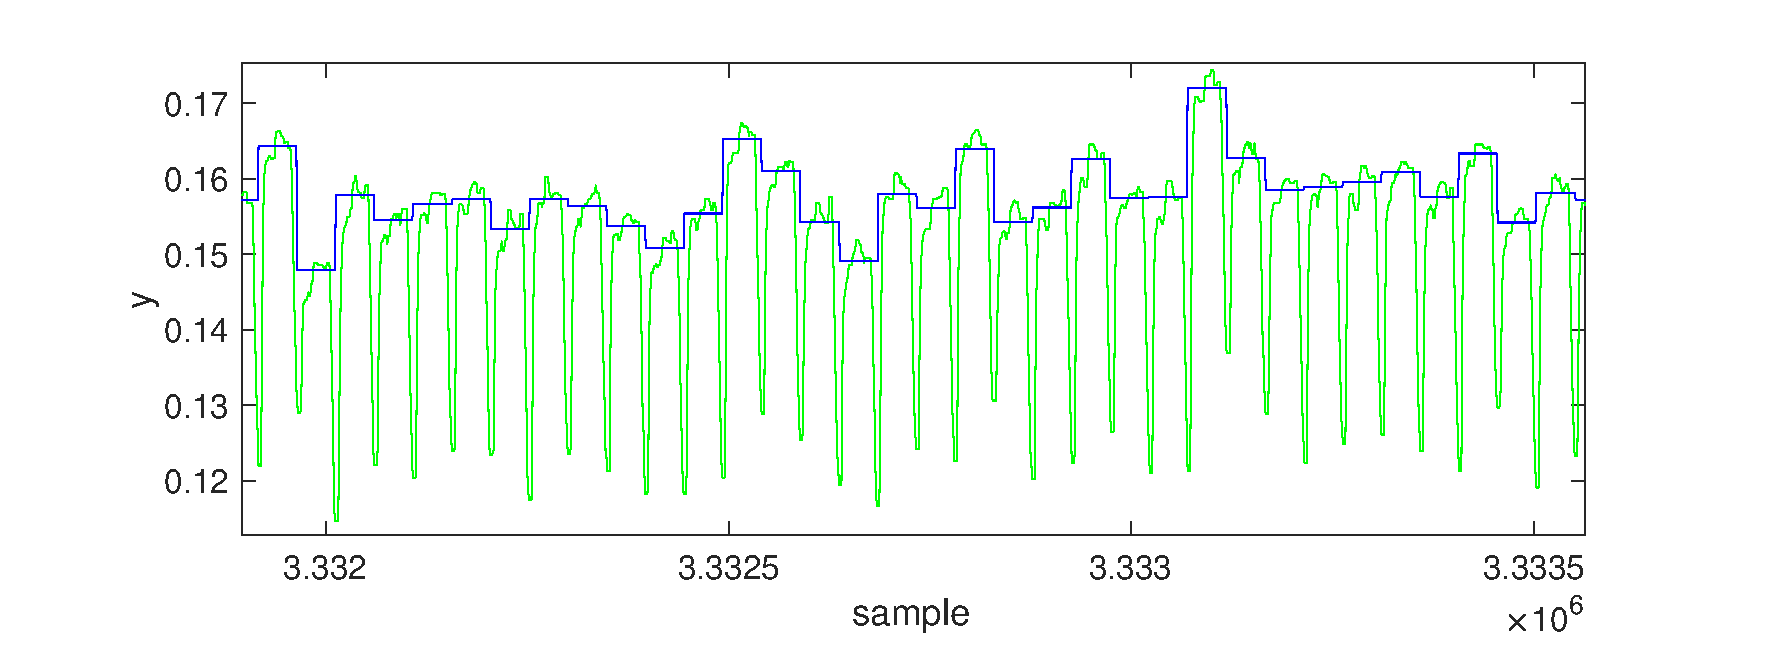
\includegraphics[width = 1\linewidth]{gfx/signal_proc/isolated_final_signal.eps}
\caption{Calculated mean value for each measurement matrix with transition measurements omitted.}
	\label{fig:detarmain_signal}
\end{figure}



\subsubsection{Dynamics in scene} %: luminance change}
\label{sec:Dynamics_in_scene}
The measured signal $\mathbf{y}$ should be stationary because the image (scene) is assumed to be static. When capturing images outdoors with natural light and long exposure times the image (or every pixel) may not be constant. This ambiguity of each pixel will reduce the reconstruction performance. The potential dynamics in a scene can be divided into two categories, luminance change and object movement. In this subsection the luminance change problem is modeled, and the corresponding algorithm will suppress the impact on the reconstructed image. The object movement problem will not be modeled, but will be avoided by ensuring that the scene is as static as possible.\\[0.1in] 


In natural outdoor images it can be assumed the primary source of light comes from the sun, but even on a clear day the light intensity from the sun is not constant. If the scene is assumed to be completely stationary, even the slightest intensity change will be amplified by all pixels being measured and thus changing the mean intensity of the measured signal $\mathbf{y}$ which should be stationary. The consequence of the sampled signal $\mathbf{y}$ not being stationary is that reconstruction performance will drop significantly. Therefore a model of light intensity change is created together with an algorithm to restore the signals stationary characteristics.\\[0.1in] 


With the assumption that the scene is constant and the luminance change is uniform over the scene, the problem can be modeled.\\[0.1in]

Start with the original theorem and disregard the noise, 

\begin{equation}
\mathbf{y} = \mathbf{\Phi}\mathbf{x}.
\end{equation}  

The image $\mathbf{x}$ can no be considered constant for all measurements, since the luminance change will change the image $\mathbf{x}$ for every measurement matrix $\mathbf{\phi}_i$. This can be described for one measurement as,  

\begin{equation}
y_i = \mathbf{\phi}_i\mathbf{x}_i = \mathbf{\phi}_i(\mathbf{x} + \mathbf{l}_i) = \mathbf{\phi}_i\mathbf{x} + \mathbf{\phi}_i\mathbf{l}_i ,
\end{equation}
  
where $\mathbf{l}_i$ uniformly adds the same intensity over the whole image $\mathbf{x}$ for measurement $i$. It is known from before that the measurement matrix $\mathbf{\phi}_i$ contains $50\%$ zeros and ones which gives,

\begin{equation}
y_i = \mathbf{\phi}_i\mathbf{x} + \mathbf{\phi}_i\mathbf{l}_i = \mathbf{\phi}_i\mathbf{x} + \frac{N}{2}c_i,
\end{equation}

where $c_i$ is the uniform intensity change coefficient for measurement $i$. This function can be generalized for all measurements,

\begin{equation}
\mathbf{y} =  \mathbf{\Phi}\mathbf{x} + \mathbf{c},
\end{equation}

where $\mathbf{c}$ is the uniform intensity change vector.\\[0.1in]

The goal is to remove the uniform intensity change vector $\mathbf{c}$ from signal $\mathbf{y}$. Using the knowledge that $\mathbf{y}$ should be stationary and assuming that the rate of change in intensity has a much lower frequency than the intensity change between individual measurement matrices, $\mathbf{c}$ can be approximated by the moving mean and removed from $\mathbf{y}$. The moving mean is calculated for each sample $\mathbf{y}[m]$ by calculating the average of $k$ samples centered around $\mathbf{y}[m]$, where $k$ i chosen depending on the DMD pattern rate.\\[0.1in]

Moving mean is defined as

\begin{equation}
\mathbf{y}_{\text{MM}}[m] = \frac{1}{k} \sum_{i = m-\frac{k+1}{2}}^{m + \frac{k+1}{2}} \mathbf{y}[i],
\end{equation}   
		 
where the calculation is made for each sample in $\mathbf{y}$ and thus the algorithm to remove uniform intensity change is,

\begin{equation}
\mathbf{y} = \mathbf{y}_{\text{SAMPLED}} - \mathbf{y}_{\text{MM}} \approx \mathbf{y}_{\text{SAMPLED}} -\mathbf{c}.
\end{equation}

The built in MATLAB function \texttt{movmean} will be used.
		 
%\subsubsection{Dynamics in scene: structure movement}
%Moving objects in the scene is more complex problem than the previous luminance change, both detecting the movement by reading the measured signal and if detected how to remove the problem. In this master's thesis scenes which is known to contain large movement will be avoided, while some small movement for example created by the wind will have to be accepted. In this section a method i proposed to detect a large object rapidly moving in and out of the scene  
%
%In this section a model of a static      

\subsubsection{Reconstruction}
Reconstruction is performed using the TVAL3 algorithm described in section~\ref{sec:TV}. The algorithm takes the measurement matrix $\mathbf{\Phi}$, the sampled signal $\mathbf{y}$ and the algorithm settings as input arguments and outputs the reconstructed image. The settings used throughout all experments is:

\begin{itemize}
\item \textit{opts.mu} = \texttt{2024}
\item \textit{opts.beta} = \texttt{64}
\item \textit{opts.maxcnt} = \texttt{10}
\item \textit{opts.maxit} = \texttt{1000}
\item \textit{opts.tol\_inn} $= 10^{-5}$
\item \textit{opts.tol} $= 10^{-10}$ 
\item \textit{opts.mu0} = \texttt{16} 
\item \textit{opts.beta0} = \texttt{1}
\item \textit{opts.nonneg} = \texttt{true}
\item \textit{opts.isreal} = \texttt{true}	
\end{itemize} 

This solves for a real non-negative solution as shown in equation~\ref{eq:tval3}. 


\subsubsection{Image processing}
\label{sec:ip}
After reconstruction of the image some simple image processing is performed. There are only two operations applied to the reconstructed image and the reason is that the presented image results should represent what can be expected from the system. Furthermore image processing is often applied on special problems or artifacts in the images and it is not desired to cover up if such artifacts exist. Therefore the only two operations used are the median filter and adjusting the intensity for higher contrast.\\[0.1in]

The reconstructed image has a high dynamic range and if only a small set of neighboring pixels is reconstructed with a high intensity peak, which not correlates with the rest of the image, these pixels will drop the contrast in the rest of the image. To remove these peaks the median filter is used. The median filter will also remove "salt and pepper" noise while edges are preserved. The built in MATLAB function \texttt{medfilt2} is be used.\\[0.1in]

The second operation is an intensity transform to maximize the contrast in the image, the built in MATLAB function \texttt{imadjust} is be used.   


\subsection{Evaluation: Image quality assessment}
\label{sec:method_eval}
The evaluation will be divided in to two categories: reconstructed images from synthetic data and images reconstructed from data acquired by the SPC.\\[0.1in] 

All results are produced with subsampling ratios ranging from 5-30\% and evaluated. The upper limit was set to 30\% partly because of the hardware limitations with long exposure time and partly because the main advantage of CS/CI is to minimize the required subsampling ratio.\\[0.1in]

The evaluation on synthetic data is focused on evaluating the performance of the measurement matrix and reconstruction algorithm. Evaluating synthetic data gives advantages that can not be achieved with images reconstructed using the SPC which is that there is a reference image which the resulting image can be compared to.\\[0.1in]

A reconstructed image from synthetic data is acquired by creating a signal $ \mathbf{ y }_{M\times1}$ taking the inner product of $ \mathbf{y} = \mathbf{\Phi} \mathbf{x} + \epsilon$ where, $\mathbf{x}$ is the synthetic image reshaped to a vector, $\mathbf{\Phi}$ is the measurement matrix with the desired amount of measurements $M$ and synthetic noise $\epsilon$ which can be regulated to simulate different conditions, then using the reconstruction algorithm on the signal $\mathbf{y}$ to obtain the reconstructed image $\mathbf{\hat x}$. Because the measurement matrix and reconstruction algorithm is independent of the SPC hardware the subsystem can be evaluated independently. Two advantages of evaluating the sensing and reconstruction independently of the SPC is that parameters such as number of measurements and noise can be regulated easy and the second advantage is that a reference image is available for comparison.\\[0.1in] 

\subsubsection{Evaluation Using reference image}
With a reference image available, two image quality assessments are performed on the result from the simulation: Peak signal-to-noise ratio (PSNR) and structural similarity (SSIM) index. PSNR is defined as

\begin{equation}
    \text{PSNR}[f(x,y),g(x,y)] = 10 \log_{10}\frac{E^2}{\text{MSE}[f(x,y),g(x,y)]}
\end{equation}
 
where, $f(x,y)$ and $g(x,y)$ are the intensity in pixel $(x,y)$, $E$ is the maximum possible pixel value and MSE is the mean square error between the images defined as

\begin{equation}
\text{MSE}[f(x,y),g(x,y)] = \frac{1}{mn}\sum_{x=0}^{m-1}\sum_{y=0}^{n-1}[f(x,y) - g(x,y)]^2.
\end{equation}

The SSIM algorithm is not focused on pixel to pixel differences like PSNR, but instead of the structure of the image in small windows. SSIM separates  luminance, contrast and structure and calculates the difference in each category in a small window to calculate the similarity of the images. The SSIM index is defined as

\begin{equation}
\text{SSIM}[f(x,y),g(x,y)] = \sum_nl[f(n),g(n)]^\alpha c[f(n),g(n)]^\beta s[f(n),g(n)]^\gamma ,
\end{equation}

where $n$ is the window, $\alpha=\beta=\gamma = 1$ and 

\begin{equation}
\displaystyle \text{luminance: } l = \frac{2\mu_{f(n)}\mu_{g(n)} + C_1}{\mu_{f(n)}^2 + \mu_{g(n)}^2 + C_1},
\end{equation}
\begin{equation}
\text{contrast: } c = \frac{2\sigma_{f(n)}\sigma_{g(n)} + C_2}{\sigma_{f(n)}^2 + \sigma_{g(n)}^2 + C_2},
\end{equation}
\begin{equation}
\text{structure: } s = \frac{\sigma_{f(n)g(n)} + C_3}{\sigma_{f(n)} \sigma_{g(n)} + C_3},
\end{equation}

where,

\begin{itemize}
\item $\mu_{f(n)}$ and $\mu_{g(n)}$ is window mean.
\item $\sigma_{f(n)}$ and $\sigma_{g(n)}$ is window standard deviation.
\item $\sigma_{f(n)g(n)}$ is window cross covariance.
\item $C_1 = 0.01*255$, (MATLAB default).
\item $C_2 = 0.03*255$, (MATLAB default).
\item $C_1 = C_2/2$, (MATLAB default).
\end{itemize} 

Which summarizes to

\begin{equation}
\text{SSIM}[f(x,y),g(x,y)] = \sum_n \frac{(2\mu_{f(n)}\mu_{g(n)} + C_1)(2\sigma_{f(n)g(n)} + C_2)}{(\mu_{f(n)}^2 + \mu_{g(n)}^2 + C_1)(\sigma_{f(n)}^2 + \sigma_{g(n)}^2 + C_2)}.
\end{equation} 

The SSIM index has a max value of 1 when the images are identical which makes it easy to read. \cite{book:image_processing}

\subsubsection{Evaluation Using no reference quality assessment}
In order to evaluate image quality when there is no reference image to compare against, the BRISQUE algorithm is used as a complement. BRISQUE is a no reference image quality assessment model which is based on natural scene statistics and quantifies the "naturalness" of the image.    \cite{article:brisque}

\subsubsection{Evaluating Using Edge response}
The edge response measures the sharpness of the image by calculating the distance in pixels required for an edge in the image to rise. In this master's thesis, the distance required for the edge response to rise from 10\% to 90\% was chosen, see figure~\ref{fig:edge_response_def}. This evaluation is performed on static images captured in constant light indoors for consistent results. Furthermore, the motive of the image is slanted geometric objects printed on a sheet of paper.\cite{article:FOI_pres_sens}
 
\begin{figure}[H]
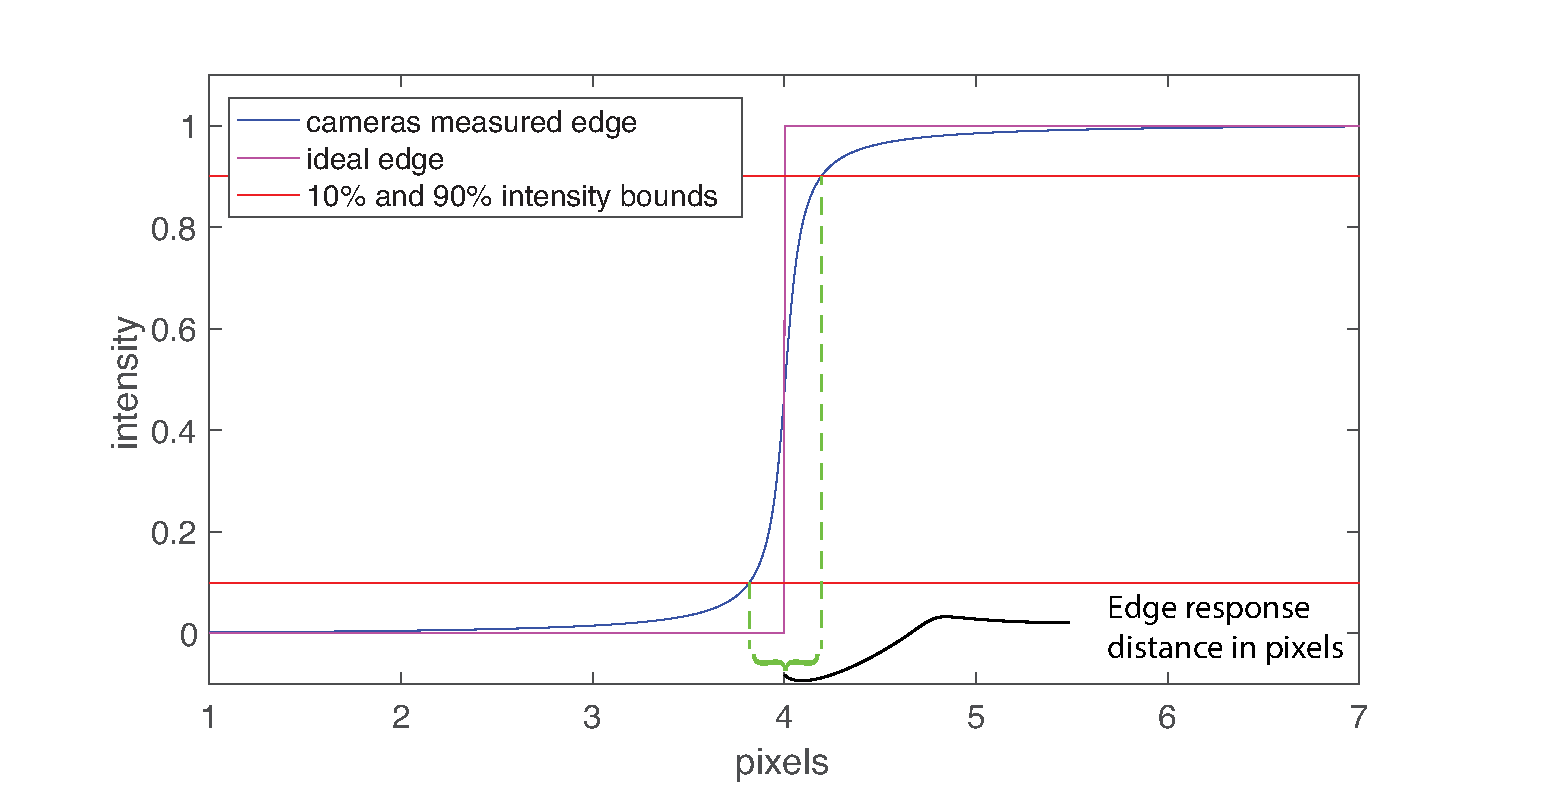
\includegraphics[width = 1\textwidth]{./result/edge_response.eps}
	\caption{Definition of 10-90\% Edge response.}
	\label{fig:edge_response_def}
\end{figure}

\pagebreak



\subsection{Method criticism}
\begin{itemize}
    \item The BRISQUE algorith is not designed for SWIR images or SPC:s characteristics noise. Therefore the results may not reflect how the quality assessment would answer to visual wavelength cameras. BRISQUE definition of "naturalness" may not reflect the images captured by the SPC. 
    \item The effect on the reconstructed images caused by the DMD mirrors alignment and pairing is not known.
\end{itemize}
%LSE - absolute error but does not say much about how humans perceives the image.\\

